\documentclass[11pt]{report}

\usepackage[utf8]{inputenc}
\usepackage{mathpazo}
  \renewcommand{\baselinestretch}{1.1}
\usepackage{amssymb}
\usepackage{amsmath}
\usepackage[font={small,it}]{caption}
\usepackage{fancyvrb}
\usepackage[letterpaper, left=1.5in, right=1.5in, top=1in, bottom=1in]{geometry}
\usepackage{hyperref}
  \hypersetup{
    breaklinks=true,
    colorlinks=true,
      anchorcolor=black,
      citecolor=black,
      filecolor=black,
      linkcolor=black,
      urlcolor=black,
    pdftitle={Bayesian Models of Gene Expression and RNA Sequencing},
    pdfauthor={Bob Carpenter, Shuonan Chen, Nikolai Vetr},
    pdfpagemode=FullScreen,
  }
\usepackage{mathtools}
\usepackage[round]{natbib}
\usepackage{sourcecodepro}
\usepackage{tikz}
  \usetikzlibrary{bayesnet,arrows,calc,patterns,positioning,shapes,snakes}
  \tikzstyle{exon}=[draw, minimum size=1.25em, minimum width=3em]
  \tikzstyle{intron}=[draw, mimimum size=1.25em minium width=1.5em, fill=gray!30]
  \tikzstyle{utr}=[exon, fill=blue!30]
  \tikzstyle{utr3}=[exon, fill=blue!30, node distance=3em]
  \tikzstyle{promoter}=[exon, fill=blue!50, minimum width=1em, node distance=2em]
  \tikzstyle{flanking}=[exon, fill=yellow!30]
  \tikzstyle{intron}=[exon, fill=gray!30]
  \tikzstyle{exon1}=[exon, fill=red!30]
  \tikzstyle{exon2}=[exon, fill=red!50]
  \tikzstyle{exon3}=[exon, fill=red!70]
  \tikzstyle{cap5}=[draw, circle, minimum size=1.5em, node distance=2.05em,  fill=orange!30]
  \tikzstyle{capsmall}=[draw, circle, minimum size=0.3em, fill=orange!30]
  \tikzstyle{bead}=[draw, circle, minimum size=1.25em, node distance=1em,  fill=green!30]
  \tikzstyle{rna}=[draw, minimum height=0.1em, minimum width=10em, fill=purple!30]
  \tikzstyle{rnafrag}=[draw, minimum height=0.1em, minimum width=2.5em, fill=purple!30]
  \tikzstyle{dnafrag}=[draw, minimum height=0.1em, minimum width=2.5em, fill=blue!30]
  \tikzstyle{polyA}=[exon, draw=none, fill=white!100, node distance=3.5em]
  \tikzstyle{textbox}=[exon, draw=none, fill=white!100, node distance=4em]
  \tikzstyle{exonB}=[draw, minimum size=0.8em, minimum width=2em]
  \tikzstyle{exon1B}=[exonB, fill=red!50]
  \tikzstyle{exon2B}=[exonB, fill=yellow!50]
  \tikzstyle{exon3B}=[exonB, fill=blue!50]
  \tikzstyle{intronB}=[exonB, fill=gray!30]
  \tikzstyle{splice}=[coordinate, node distance=1.5em]
  \tikzset{%
    body/.style={inner sep=0pt,outer sep=0pt,shape=rectangle,draw,thick,pattern=north east lines wide},
    dimen/.style={<->,>=latex,thin,every rectangle node/.style={fill=white,midway,font=\sffamily}},
    symmetry/.style={dashed,thin},
  }
% 15\usepackage{tocbibind}
\usepackage{verbatimbox}
\usepackage{xspace}

% basic math
\newcommand{\logit}{\textrm{logit}}
\newcommand{\ilogit}{\logit^{-1}}
\newcommand{\rngto}[1]{1{:}#1}
\newcommand{\setlist}[1]{\{ #1 \}}
\newcommand{\setcomp}[2]{\{ #1 \, : \, #2 \}}
\newcommand{\deriv}[1]{\frac{\textrm{d}}{\textrm{d}#1}}
\newcommand{\indicator}[1]{\textrm{I}\!\left( #1 \right)}
\newcommand{\vect}[1]{[#1]^{\top}}

% basic prob
\newcommand{\distro}[3]{\textrm{#1}\!\left( #2 \,|\, #3\right)}
\newcommand{\distrobig}[3]{\textrm{#1}\!\left( #2 \,\bigg|\, #3\right)}
\newcommand{\rdistro}[2]{\textrm{#1}\!\left( #2 \right)}
\newcommand{\pone}[1]{p\!\left( #1 \right)}
\newcommand{\p}[2]{\pone{#1 \,|\, #2}}


% constants
\newcommand{\mybase}[1]{\texttt{#1}\xspace}
\newcommand{\baseA}{\mybase{A}}
\newcommand{\baseC}{\mybase{C}}
\newcommand{\baseG}{\mybase{G}}
\newcommand{\baseT}{\mybase{T}}
\newcommand{\baseU}{\mybase{U}}
\newcommand{\baseY}{\mybase{Y}}
\newcommand{\baseN}{\mybase{N}}
\newcommand{\baseR}{\mybase{R}}


% formatting
\newcommand{\stancode}[1]{\verbfilebox[\small]{../../stan/#1}\theverbbox}
\newcommand{\mycaption}[2]{\caption{#2}\label{#1}}
\newcommand{\anitem}[1]{\begin{itemize} \item #1 \end{itemize}}

\setlength{\floatsep}{24pt}

\title{Bayesian Models of Gene Expression and RNA Sequencing}
\author{Bob Carpenter \\ Flatiron Institute
  \and Shuonan Chen \\ Columbia University
  \and Nikolai G.\ Vetr \\ Stanford University}
\date{\the\year-\the\month-\the\day \ (Draft)}

\begin{document}

\maketitle

\begin{abstract}
  \noindent
  We develop a fully Bayesian, generative approach to RNA sequencing
  (RNA-seq) data.  We start with a simple binomial model and
  incrementally expand it to deal with alignment uncertainty, technical
  and biological variation in replicated samples, and differential
  expression among grouped samples.  We introduce multinomial, log, and,
  logistic parameterizations of expected reads and derive the relation
  among multinomial, binomial, Poisson, and negative binomial models of
  read counts. We model expression hierarchically at the group level and
  use partially pooled replicate-level effects to model technical and
  biological variation among replicates.  By treating the alignment of
  multi-aligned reads as a discrete random variable, we can model the
  expression of exons, isoforms, or genes.  Probabilistic inference for
  quantities of interest, such as log fold change between the
  group-level expression of an isoform, follows directly.  We
  demonstrate the robustness of posterior predictive inference in the
  face of limited data, noisy data, and unidentifiable parameters.
\end{abstract}

\tableofcontents

\chapter{Introduction}

We are primarily interested in estimating the relative expression of
genes, exons, or isoforms from RNA sequencing (RNA-seq) data which has
been collected from multiple biologically distinctive groups, with
replicated samples from each group.  The replicates may consist of
multiple cells from a single subject or samples from multiple
subjects.  Our inferential goal is to estimate group-level and
replicate-level expression, from which we can derive probabilities of
differential expression.

Dozens of tools exist to estimate differential expression at the group
level, so it is natural to ask why we are proposing one more.  The
short answer is that almost all of the popular tools that people use
like DESeq2 \citep{love2014differential} or rMATS \citep
{shen2014rmats}, employ heuristic empirical Bayes techniques to
compute an approximate maximum marginal likelihood estimate, followed
by frequentist significance testing for the null hypothesis of no or
small differences in expression.  In contrast, we will present a fully
Bayesian approach that is general enough to encapsulate most of the
models that have been proposed in the literature.

\cite{lewin2019bayesian} provide an excellent overview of Bayesian
differential expression modeling.  Our presentation here is consistent
with theirs, but even more elementary in terms of what it presupposes
of readers in terms of cellular biology or Bayesian statistics.  For
all of the models we discuss, we provide reproducible Stan programs
and R scripts to simulate data and fit models.\footnote{All of our
  code is available from GitHub and open-source licensed. See
  \url{https://github.com/bob-carpenter/BayesExpress}.}


\chapter{DNA, RNA, and Proteins}

We begin with a short overview of RNA sequencing (RNA-seq) technology,
because it will motivate the models we are proposing.  First, we cover
the \textit{in vivo} process of mRNA being transcribed from the genome
and spliced into mRNA.  Second, we describe the \textit{in vitro}
process of enrichment, fragmentation, reverse transcription,
amplification, and sequencing.  The final section describes the
\textit{in silico} process of alignment of the reads to the genome and
expression modeling.

Samples used for RNA-seq may be drawn from a single cell or from a
mixture of cells.  Samples are often organized into groups, such as
wild-type vs.\ cancerous liver cells, or at an even finer grain, with
individual neural cell types.  There are hundreds of human cell types
and cells of a given type change state over time.  In addition, there
is an intrinsic reduction in variability in averaging as shown by the
central limit theorem.  As a result of these two factors, single-cell
RNA-seq data is much more heterogeneous than mixture data.

The process we describe below is a standard one from Illumina, a very
widely used sequencing platform \cite{quail2008large}.  Although we
present a standard process, even the Illumina sequencer allows a wide
range of variation in sample preparation and sequencing used.

\begin{figure}[t!]
  \centering
  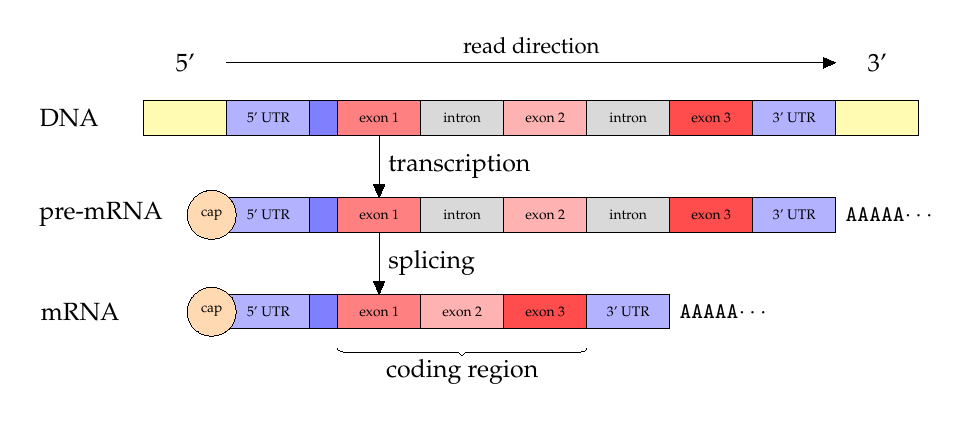
\begin{tikzpicture}[node distance=3em, line width=0mm]
    \node(nc5) [flanking] {};
    \node(utr5) [utr, right of=nc5] {\tiny 5' UTR};
    \node(p) [promoter, right of=utr5] {};
    \node (a1) [exon2, right of=p, node distance=2em] {\tiny exon 1};
    \node (i1) [intron, right of = a1] {\tiny intron};
    \node (a2) [exon1, right of=i1] {\tiny exon 2};
    \node (i2) [intron, right of=a2] {\tiny intron};
    \node (a3) [exon3, right of=i2] {\tiny exon 3};
    \node (utr3) [utr3, right of=a3] {\tiny 3' UTR};
    \node (nc3) [flanking, right of=utr3] {};
    \node (text1) [textbox, left of=nc5, xshift=-0.2em] {\small DNA};
    %
    \node (Butr5) [utr, below of=utr5, node distance=3.5em] {\tiny 5' UTR};
    \node (Bp) [promoter, right of=Butr5] {};
    \node (Ba1) [exon2, right of=Bp, node distance=2em] {\tiny exon 1};
    \node (Bi1) [intron, right of = Ba1] {\tiny intron};
    \node (Ba2) [exon1, right of=Bi1] {\tiny exon 2};
    \node (Bi2) [intron, right of=Ba2] {\tiny intron};
    \node (Ba3) [exon3, right of=Bi2] {\tiny exon 3};
    \node (Butr3) [utr3, right of=Ba3] {\tiny 3' UTR};
    \node (BpolyA) [polyA, right of=Butr3] {\footnotesize \texttt{AAAAA}$\cdots$};
    \node (cap) [cap5, left of=Butr5] {\tiny cap};
    \node (text2) [textbox, left of=cap] {\small pre-mRNA};
    %
    \node (Cutr5) [utr, below of=Butr5, node distance=3.5em] {\tiny 5' UTR};
    \node (Cp) [promoter, right of=Cutr5] {};
    \node (Ca1) [exon2, right of=Cp, node distance=2em] {\tiny exon 1};
    \node (Ca2) [exon1, right of=Ca1] {\tiny exon 2};
    \node (Ca3) [exon3, right of=Ca2] {\tiny exon 3};
    \node (Cutr3) [utr3, right of=Ca3] {\tiny 3' UTR};
    \node (CpolyA) [polyA, right of=Cutr3] {\footnotesize\texttt{AAAAA}$\cdots$};
    \node (Ccap) [cap5, left of=Cutr5] {\tiny cap};
    \node (text2) [textbox, left of=Ccap, xshift=-0.75em] {\small mRNA};

    \node (start5) [textbox, above of=nc5, node distance=2em] {\small 5'};
    \node (end3)  [textbox, above of=nc3, node distance=2em] {\small 3'};
    \draw [->] (start5) -- (end3) node[midway, above] {\footnotesize read direction};
    \draw [->] (a1) -- (Ba1) node[midway, right] {\small transcription};
    \draw [->] (Ba1) -- (Ca1) node[midway, right] {\small splicing};
    \draw [decoration={brace, mirror, raise=0.25cm}, decorate] (Ca1.south west) -- (Ca3.south east)
    node [pos=0.5,anchor=north,yshift=-0.75em] {\small coding region};
  \end{tikzpicture}
  \mycaption{fig:transcriptome-splicing}{Sketch of the \textit{in
      vivo} cellular process that produces mature mRNA through
    transcription and splicing.  DNA (top) is transcribed to pre-mRNA
    (middle); this process starts with the 5' untranslated region
    (UTR) and ends with the 3' UTR.  The dark blue section of the 5'
    UTR indicates the promoter region that is used to regulate the
    transcription process.  After transcription, the pre-mRNA is
    capped on the 5' end and polyadenylated on the 3' end.  The
    introns are then spliced out of the pre-mRNA to form mRNA
    (bottom).  Only the coding region consisting of the exon sequence
    is translated to a sequence of amino acids by the ribosome.}
\end{figure}

\begin{figure}[t!]
  \centering
  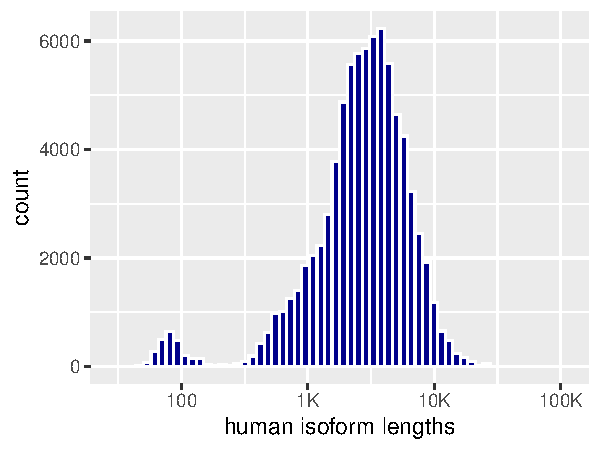
\includegraphics[width=2.5in]{../../img/isoform-human-length-histogram.pdf}
  \mycaption{fig:iso-lengths}{Histogram of lengths of the coding
    region of human isoforms, with the $x$-axis on a log scale. The
    transcriptome used is version GRCh38 of the Reference Sequence
    Database Transcripts (RefSeq Transcripts) supplied by the U.S.\
    National Center for Biotechnology Information (NCBI)
    \citep{oleary2016reference}. Only the 80,791 curated isoforms are
    used (i.e., those not marked {\small \texttt{PREDICTED}).}}
\end{figure}

\section{From DNA to mRNA}

A cell's DNA is arranged into chromosomes, each of which consists of a
two strands of nucleotides with opposite orientations arranged in a
double helix. The bases of these nucleotides are adenine (\baseA),
cytosine (\baseC), guanine (\baseG), and thiamine (\baseT). The bases
are attached to an alternating sugar-phosphate backbone which is
oriented with sugar-phosphate bonds at the 5' and 3' atoms of the
sugar ring.

A gene consists of a structured subsequence of bases that begins on
the 5' end with an untranslated region (5' UTR) that is involved in
regulating and initiating a gene's transcription. A gene ends on a 3'
end with a second untranslated region (3' UTR).
\citep{mignone2002untranslated} provide a detailed overview of the
structure and function of the 5' and 3' untranslated regions of a
gene. The central portion of a gene is a sequence of exons separated
by introns. The sketch of the sequence making up a gene is illustrated
in the top line of Figure~\ref{fig:transcriptome-splicing}

During the transcription process, mRNA is transcribed from the DNA,
capped on the 5' end, and polyadenylated on the 3' end with a sequence
of adenine (\baseA) bases known as the poly(A) tail. The resulting
pre-mRNA is shown on the second line of
Figure~\ref{fig:transcriptome-splicing}.

Finally, the introns and possibly some exons are spliced out of the
pre-mRNA to produce the final mRNA, as shown in the bottom line of
Figure~\ref{fig:transcriptome-splicing}. The splicing operation is
often non-deterministic in higher eukaryotes; in humans, most genes
produce multiple splice variants known as isoforms. The final result
of transcription and splicing is mature mRNA, which is then translated
to a polypeptide (i.e., a sequence of amino acids), which then folds
into a protein.

Figure~\ref{fig:iso-lengths} provides a histogram of human isoform
lengths. These lengths vary widely, with the shortest being 33 bases
and the longest 109,224 bases. The median number of bases in an
isoform is 2879, the central 50\% interval is (1714, 4568) and the
central 95\% interval is (100, 10187). The mean isoform length is 3506
and the sample standard deviation is 2856.

We are interested in expression because the genes and isoforms
expressed by a cell determine the cell's function. By studying
differential expression of RNA among cells of different types, we hope
to uncover clues about cell regulation and differentiation.

\section{From mRNA to protein}

\begin{table}[t!]
  \centering\small
  \setlength\doublerulesep{4pt}
  \setlength{\tabcolsep}{4pt}
  \centering\small
  \begin{tabular}{|ccc|c|}
    \hline
    \multicolumn{3}{|c|}{\textit{codon}} & \textit{acid}
    \\ \hline \hline
    \baseU & \baseU & \baseU & phe
    \\ &        & \baseC &
    \\ \hline
    &  & \baseA & leu
    \\ & & \baseG &
    \\ \hline \hline
    \baseC & \baseU & \baseU & leu
    \\ & & \baseC &
    \\ & & \baseA &
    \\ & & \baseG &
    \\ \hline \hline
    \baseA & \baseU & \baseU & ile
    \\ & & \baseC &
    \\ & & \baseA &
    \\ \hline
    &  & \baseG & met$^*$
    \\ \hline \hline
    \baseG & \baseU & \baseU & val
    \\ & & \baseC &
    \\ & & \baseA &
    \\ & & \baseG &
    \\ \hline
  \end{tabular}
  \qquad
  \begin{tabular}{|ccc|c|}
    \hline
    \multicolumn{3}{|c|}{\textit{codon}} & \textit{acid}
    \\ \hline \hline
    \baseU & \baseC & \baseU & ser
    \\ & & \baseC &
    \\ & & \baseA &
    \\ & & \baseG &
    \\ \hline \hline
    \baseC & \baseC & \baseU & pro
    \\ & & \baseC &
    \\ & & \baseA &
    \\ & & \baseG &
    \\ \hline \hline
    \baseA & \baseC & \baseU & thr
    \\ & & \baseC &
    \\ & & \baseA &
    \\ & & \baseG &
    \\ \hline \hline
    \baseG & \baseC & \baseU & ala
    \\ & & \baseC &
    \\ & & \baseA &
    \\ & & \baseG &
    \\ \hline
  \end{tabular}
  \qquad
  \begin{tabular}{|ccc|c|}
    \hline
    \multicolumn{3}{|c|}{\textit{codon}} & \textit{acid}
    \\ \hline \hline
    \baseU & \baseA & \baseU & tyr
    \\ & & \baseC &
    \\ \hline
    &  & \baseA & \textit{stop}
    \\ & & \baseG &
    \\ \hline \hline
    \baseC & \baseA & \baseU & his
    \\ & & \baseC &
    \\ \hline
    &  & \baseA & gln
    \\ & & \baseG &
    \\ \hline \hline
    \baseA & \baseA & \baseU & asp
    \\ & & \baseC &
    \\ \hline
    &  & \baseA & lys
    \\ & & \baseG &
    \\ \hline \hline
    \baseG & \baseA & \baseU & asp
    \\ & & \baseC &
    \\ \hline
    &  & \baseA & glu
    \\ & & \baseG &
    \\ \hline
  \end{tabular}
  \qquad
  \begin{tabular}{|ccc|c|}
    \hline
    \multicolumn{3}{|c|}{\textit{codon}} & \textit{acid}
    \\ \hline \hline
    \baseU & \baseG & \baseU & cys
    \\ & & \baseC &
    \\ \hline
    &  & \baseA & \textit{stop}
    \\ \hline
    &  & \baseG & trp
    \\ \hline \hline
    \baseC & \baseG & \baseU & arg
    \\ & & \baseC &
    \\ & & \baseA &
    \\ & & \baseG &
    \\ \hline \hline
    \baseA & \baseG & \baseU & ser
    \\ & & \baseC &
    \\ \hline
    &  & \baseA & arg
    \\ & & \baseG &
    \\ \hline \hline
    \baseG & \baseG & \baseU & gly
    \\ & & \baseC &
    \\ & & \baseA &
    \\ & & \baseG &
    \\ \hline
  \end{tabular}
  \mycaption{tab:genetic-code}{A figure representing the genetic code,
    which is a mapping from codons consisting of three RNA bases
    (\baseU, \baseC, \baseA, and \baseG) to amino acids and the stop
    signal. The boxes represent the initial two bases, with each row
    sharing the same first base and each column the same second base.
    A single codon encodes tryptophan (trp), whereas six encode
    leucine (leu). The codon \baseA~\baseU~\baseG encodes the amino
    acid methionine (met) and also signals the start of translation. }
\end{table}
%
The ribosome, a molecule composed of ribosomal RNA (rRNA) and
proteins, coordinates the translation of the mRNA to a sequence of
amino acids that will make up a protein. The mRNA is arranged into
groups of three bases, called codons, each of which translates to an
amino acid (one of which does double duty as the start signal), or end
signal. There are 20 distinct amino acids. The genetic code, shown in
Table~\ref{tab:genetic-code}, is the mapping from codons to amino
acids and the stop signal. With $4^3 = 64$ codons and only 20 amino
acids (including one doing double-duty as the start signal) plus the
stop signal, there are cases where more than one codon maps to the
same amino acid. For example, the codons \baseU{}\baseU{}\baseU and
\baseU{}\baseU{}\baseC both translate to the amino acid phenylalanine
(phe), and the codons \baseU{}\baseA{}\baseA, \baseU{}\baseA{}\baseG,
and \baseU{}\baseG{}\baseA all provide a stop signal.

\begin{figure}[t]
  \centering
  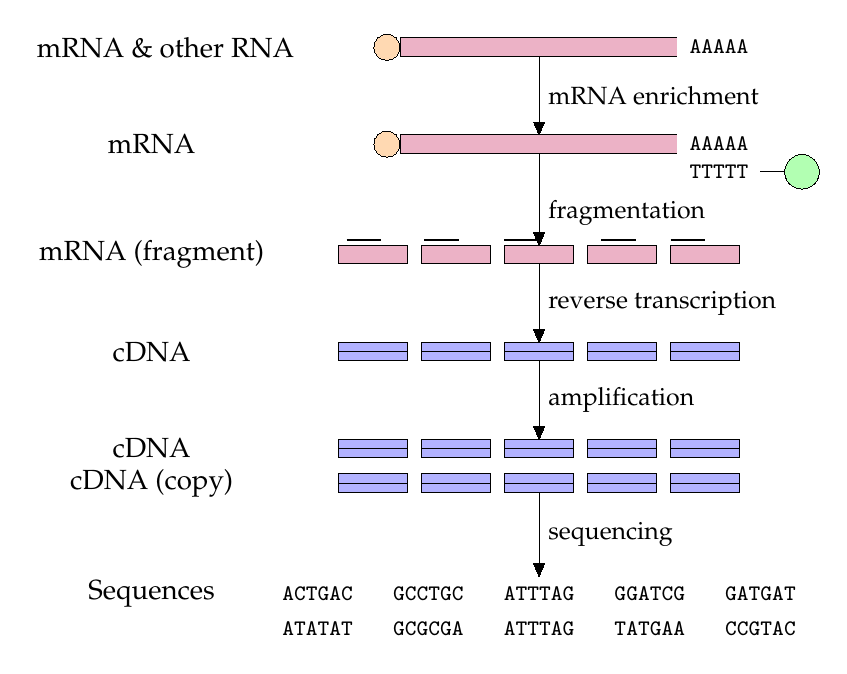
\begin{tikzpicture}[node distance=3em, line width=0mm]
    \node (cap1) [capsmall] {};
    \node (rna1) [rna, right of=cap1, node distance=5.5em] {};
    \node (polyA1) [polyA, right of=rna1, node distance=6.5em] {\footnotesize \texttt{AAAAA}};
    %
    \node (cap2) [capsmall, below of=cap1, yshift=-0.5em] {};
    \node (rna2) [rna, right of=cap2, node distance=5.5em] {};
    \node (polyA2) [polyA, right of=rna2, node distance=6.5em] {\footnotesize \texttt{AAAAA}};
    \node (polyT2) [polyA, below of=polyA2, node distance=1em] {\footnotesize \texttt{TTTTT}};
    \node (bead2) [bead, right of=polyT2, node distance=3em] {};
    \draw [-] (polyT2) -- (bead2) {};
    %
    \node (frag1) [rnafrag, below of=cap2, xshift=-0.5em, yshift=-1em] {};
    \node (frag2) [rnafrag, right of=frag1] {};
    \node (frag3) [rnafrag, right of=frag2] {};
    \node (frag4) [rnafrag, right of=frag3] {};
    \node (frag5) [rnafrag, right of=frag4] {};
    \draw [-, thick] ([yshift=0.2em, xshift=0.3em]frag1.north west) -- ([yshift=0.2em, xshift=0.3em]frag1.north) {};
    \draw [-, thick] ([yshift=0.2em, xshift=0.1em]frag2.north west) -- ([yshift=0.2em, xshift=0.1em]frag2.north) {};
    \draw [-, thick] ([yshift=0.2em]frag3.north west) -- ([yshift=0.2em]frag3.north) {};
    \draw [-, thick] ([yshift=0.2em, xshift=0.5em]frag4.north west) -- ([yshift=0.2em, xshift=0.5em]frag4.north) {};
    \draw [-, thick] ([yshift=0.2em]frag5.north west) -- ([yshift=0.2em]frag5.north) {};
    %
    \node (dna1) [dnafrag, below of=frag1, yshift=-0.5em] {};
    \draw [-] (dna1.west) -- (dna1.east) {};
    \node (dna2) [dnafrag, right of=dna1] {};
    \draw [-] (dna2.west) -- (dna2.east) {};
    \node (dna3) [dnafrag, right of=dna2] {};
    \draw [-] (dna3.west) -- (dna3.east) {};
    \node (dna4) [dnafrag, right of=dna3] {};
    \draw [-] (dna4.west) -- (dna4.east) {};
    \node (dna5) [dnafrag, right of=dna4] {};
    \draw [-] (dna5.west) -- (dna5.east) {};
    %
    \node (dna1b) [dnafrag, below of=dna1, yshift=-0.5em] {};
    \draw [-] (dna1b.west) -- (dna1b.east) {};
    \node (dna2b) [dnafrag, right of=dna1b] {};
    \draw [-] (dna2b.west) -- (dna2b.east) {};
    \node (dna3b) [dnafrag, right of=dna2b] {};
    \draw [-] (dna3b.west) -- (dna3b.east) {};
    \node (dna4b) [dnafrag, right of=dna3b] {};
    \draw [-] (dna4b.west) -- (dna4b.east) {};
    \node (dna5b) [dnafrag, right of=dna4b] {};
    \draw [-] (dna5b.west) -- (dna5b.east) {};
    %
    \node (dna1c) [dnafrag, below of=dna1b, yshift=1.75em] {};
    \draw [-] (dna1c.west) -- (dna1c.east) {};
    \node (dna2c) [dnafrag, right of=dna1c] {};
    \draw [-] (dna2c.west) -- (dna2c.east) {};
    \node (dna3c) [dnafrag, right of=dna2c] {};
    \draw [-] (dna3c.west) -- (dna3c.east) {};
    \node (dna4c) [dnafrag, right of=dna3c] {};
    \draw [-] (dna4c.west) -- (dna4c.east) {};
    \node (dna5c) [dnafrag, right of=dna4c] {};
    \draw [-] (dna5c.west) -- (dna5c.east) {};
    %
    \node (seq3) [textbox, below of=dna3c] {\footnotesize\tt ATTTAG};
    \node (seq4) [textbox, right of=seq3] {\footnotesize\tt GGATCG};
    \node (seq5) [textbox, right of=seq4] {\footnotesize\tt GATGAT};
    \node (seq2) [textbox, left of=seq3] {\footnotesize\tt GCCTGC};
    \node (seq1) [textbox, left of=seq2] {\footnotesize\tt ACTGAC};
    %
    \node (seq3b) [textbox, below of=seq3, yshift=2.75em] {\footnotesize\tt ATTTAG};
    \node (seq4b) [textbox, right of=seq3b] {\footnotesize\tt TATGAA};
    \node (seq5b) [textbox, right of=seq4b] {\footnotesize\tt CCGTAC};
    \node (seq2b) [textbox, left of=seq3b] {\footnotesize\tt GCGCGA};
    \node (seq1b) [textbox, left of=seq2b] {\footnotesize\tt ATATAT};

    \node (label1) [textbox, left of=seq3, xshift=-10em] {Sequences};
    \node (label2) [textbox, left of=dna1c, xshift=-4em] {cDNA (copy)};
    \node (label3) [textbox, left of=dna1b, xshift=-4em] {cDNA};
    \node (label4) [textbox, left of=dna1, xshift=-4em] {cDNA};
    \node (label5) [textbox, left of=frag1, xshift=-4em] {mRNA (fragment)};
    \node (label6) [textbox, left of=cap2, xshift=-4.5em] {mRNA};
    \node (label7) [textbox, left of=cap1, xshift=-4em] {mRNA \& other RNA};
    %
    \draw [->] (rna1) -- (rna2) node[midway, right] {\small mRNA enrichment};
    \draw [->] (rna2) -- (frag3) node[midway, right, yshift=-0.5em] {\small fragmentation};
    \draw [->] (frag3) -- (dna3) node[midway, right] {\small reverse transcription};
    \draw [->] (dna3) -- (dna3b) node[midway, right] {\small amplification};
    \draw [->] (dna3c) -- (seq3) node[midway, right] {\small sequencing};
  \end{tikzpicture}
  \mycaption{fig:cDNA-synthesis}{Sketch of the \emph{in vitro} laboratory process for a typical RNA sequencing experiment.  The first step, poly(A) selection, uses magnetic beads to bind to the poly(A) tails of mRNA to enrich it relative to other RNA such as ribosomal RNA (rRNA) or microRNA (miRNA).  The second step, fragmentation by random hexamers, introduces random short oligo-DNA sequences that anneal at multiple points along the mRNA transcript and serve as primers for reverse transcription.  Reverse transcription synthesizes double-stranded cDNA from the mRNA fragments.  These double-stranded cDNA fragments are then amplified with a polymerase chain reaction (PCR).  In the final step, the sequencer ``reads'' the bases of the cDNA fragments and reports them as a sequence of characters.}
\end{figure}

\chapter{RNA Sequencing \& Alignment}

\section{Reverse transcription and sequencing}

Because sequencers work on short sequences of double-stranded cDNA, an
mRNA sample must be fragmented and reverse transcribed before
sequencing. To filter a biological sample to the mRNA to reverse
transcribe, either the the poly(A) tails of mRNA are selected or the
ribosomic RNA is depleted from the sample. The remaining mRNA is then
fragmented and then primed for reverse transcription using either
oligo(dT) priming or random hexamer primers. Oligo(dT) priming is
heavily biased toward the 3' end of the mRNA because it binds to the
poly(A) tail of mRNA. Random hexamers are biased to such an extent
that initial hexamer counts can vary by an two orders of magnitude.
The primed mRNA is then reverse transcribed to cDNA.

After being reverse transcribed from the mRNA fragments, the
synthesized cDNA is sequenced. The Illumina sequencing process is
based on imaging of complementary nucleotides tagged with fluorescent
markers. Imaging software then makes the call as to which base was
present on the cDNA. For short single reads on the order of 100 bases,
the Illumina sequencing process has 99\% or more accuracy per base,
with accuracy declining along the sequence~\citep{tan2019long}.

Most sequencing technologies produces reads on the order of 100 bases
long. Long-read sequencing (LRS) technology, such as single-molecule
real-time sequencing \citep{ardui2018single} from Pacific Biosciences
and nanopore sequencing from Oxford Nanopores Technology
\citep{deamer2016three}, can sequence up to 10,000 bases. These bases
require an entirely different paradigm of analysis due to higher error
rates and the fact that most mRNA is shorter than 10,000 bases. In
addition to a higher error rate, long-read sequencing has lower
throughput and requires fresh samples to avoid mRNA degradation
\citep{mantere2019long}.

\section{Alignment}

For all of the analyses we discuss here, we will assume that a
reference genome sequence or transcriptome sequence is available. A
reference genome is a set of reference chromosomes, each of which is
represented as a sequence of bases including genes and other genetic
material, with the genes being further subdivided into a sequence of
exons and introns. A reference transcriptome is a set of reference
isoforms, each of which consists of a sequence of exons.

\begin{table}[t!]
  \centering\small
  \begin{tabular}{r|cccccccccccccc}
    \textit{read} &  & & & \baseA & \baseG & \baseT & \baseT & \baseC & \baseA & \baseG &
    \\
    \textit{reference} & $\cdots$ & $\cdots$ & \baseG & \baseA & \baseG & \baseT & \baseT & \baseC & \baseA & \baseG & \baseG & $\cdots$ & $\cdots$
    \\ \hline
    \textit{exons} & $\cdots$ & \multicolumn{11}{|c|}{exon 1} & $\cdots$
  \end{tabular}
  \\[12pt]
  \begin{tabular}{r|ccccccccccccccc}
    \textit{read} &  & & & \baseA & \baseG & \baseT & & \baseT & \baseC & \baseA & \baseG &
    \\
    \textit{reference} & $\cdots$ & $\cdots$ & \baseG & \baseA & \baseG & \baseT & $\cdots$ & \baseT & \baseC & \baseA & \baseG & \baseG & $\cdots$ & $\cdots$
    \\ \hline
    \textit{exons} & $\cdots$ & \multicolumn{5}{|c|}{exon 1} & intron
                         & \multicolumn{6}{|c|}{exon 2}
  \end{tabular}
  \\[12pt]
  \begin{tabular}{r|ccccccccccccccc}
    \textit{read} &  & & & \baseA & \baseG & \baseT & \baseT & \baseC & \baseA & \baseG &
    \\
    \textit{reference} & $\cdots$ & $\cdots$ & \baseG & \baseA & \baseG & \baseT & \baseT & \baseC & \baseA & \baseG & \baseG  & $\cdots$ & $\cdots$
    \\ \hline
    \textit{exons} & $\cdots$ & \multicolumn{5}{|c|}{exon 1}
                       & \multicolumn{6}{|c|}{exon 2}
  \end{tabular}
  \mycaption{tab:split-align}{Examples of aligning mRNA reads to the
    genome and transcriptome. Reads may align to the genome or
    transcriptome fully within an exon (top). Alignments of reads to
    the genome may cross exon junctions (middle). Alignment of
    cross-exon reads to the transcriptome does not require splitting
    (bottom).}
  \label{tab:my_label}
\end{table}

The first step of \textit{in silico} analysis is to align each read,
consisting of a short sequence of called bases, to a reference genome
or reference transcriptome. When aligning to the genome, mRNA
fragments may cross exon junctions, which complicates genome alignment
algorithms and results. Alignment to the transcriptome does not
require splitting the reads, but ambiguous reads are much more
prevalent due to repeated sequences of exons across isoforms.
Table~\ref{tab:split-align} illustrates alignments within and across
exons in the genome and transcriptome.

The bases in a reference genome or transcriptomes are merely a sketch,
known as a consensus sequence, of what an individual's genome might
look like. Human genomes vary at a rate of roughly one base per
thousand, with most variation being in the form of single nucleotide
polymorphisms (SNPs), which involve the substitution, insertion, or
deletion of a single base. Table~\ref{tab:edit-distance} shows example
alignments involving a single substitution, deletion, or insertion.

\begin{table}[t!]
  \centering
  \begin{tabular}{c|c|c}
    \textit{type} & \textit{effect} & \textit{example}
    \\ \hline
    synonymous & same amino acid & \baseU{}\baseU{}\baseU $\rightarrow$ \baseU{}\baseU{}\baseC
    \\
                  & & \baseU{}\baseU{}\baseA{} $\rightarrow$ \baseC{}\baseU{}\baseA
    \\ \hline
    missense & different amino acid & \baseC{}\baseA{}\baseU $\rightarrow$ \baseC{}\baseA{}\baseA
    \\
                  & & \baseC{}\baseA{}\baseU $\rightarrow$ \baseC{}\baseC{}\baseU
    \\
                  & & \baseC{}\baseA{}\baseU $\rightarrow$ \baseG{}\baseA{}\baseU
    \\ \hline
    nonsense & stop signal & \baseC{}\baseA{}\baseA{} $\rightarrow$ \baseU{}\baseA{}\baseA{}
    \\
                  & & \baseU{}\baseC{}\baseA $\rightarrow$ \baseU{}\baseG{}\baseA
    \\
                  & & \baseU{}\baseA{}\baseC $\rightarrow$ \baseU{}\baseA{}\baseG
  \end{tabular}
  \mycaption{tab:snp-types}{There are three possible effects of a singular nucleotide polymorphism.}
\end{table}

Substitution of bases within a codon have three different types of
effects. A synonymous substitution is one in which the amino acid
being coded does not change. For example, \baseU{}\baseC{}\baseU and
\baseU{}\baseC{}\baseA both code for serine, so substituting \baseU
for \baseA in the third position of a codon beginning with
\baseU{}\baseC is an example of a synonymous substitution. Synonymous
substitutions may nevertheless cause differences in expression because
of differences in translation efficiency. A missense substitution
causes the wrong amino acid to be coded. For example, because
\baseU\baseU\baseU codes phenylalanine and \baseU{}\baseC{}\baseU
codes serine, substituting \baseU for \baseC in the second position
here results in a missense substitution. A nonsense substitution turns
a codon that codes for an amino acid into a stop codon. For instance,
\baseC{}\baseA{}\baseA codes for glutamine (gln), whereas
\baseU{}\baseA{}\baseA is the stop codon, so a substitution of \baseU
for \baseC in the first position of a codon ending in \baseA{}\baseA
results in a nonsense substitution.

\begin{table}[t!]
  \centering\small
  \begin{tabular}{r|cccccccccccl}
    \textit{read} & & \baseG & \baseA & \baseG & \baseT & \baseT & \baseC & \baseA & \baseG
    \\
    \textit{reference} & $\cdots$ & \baseG & \baseA & \baseG & \baseC & \baseT & \baseC & \baseA & \baseG & $\cdots$
    \\ \hline
    \textit{edits} &  & - & - & - & \small S & - & - & - & - &  & \small (distance 1, substitute)
  \end{tabular}
  \\[12pt]
  \begin{tabular}{r|ccccccccccccl}
    \textit{read} & & \baseG & \baseA &\baseT & \baseG & \baseT & \baseT & \baseC & \baseA & \baseG &
    \\
    \textit{reference} & $\cdots$ & \baseG & \baseA & \baseT & \baseG & \baseT & \baseT & \baseC & $\bullet$ & \baseG & $\cdots$
    \\ \hline
    \textit{edits} & & - & - & - & - & - & - & - & \small I & - & & \small (distance 1, insert)
  \end{tabular}
  \\[12pt]
  \begin{tabular}{r|ccccccccccccl}
<    \textit{read} & & \baseG & $\bullet$ & \baseC & \baseG & \baseT & \baseT & \baseC & \baseA & \baseG &
    \\
    \textit{reference} & $\cdots$ & \baseG & \baseA & $\baseC$ & \baseG & \baseT & \baseT & \baseC & \baseA & \baseG & $\cdots$
    \\ \hline
    \textit{edits} & & - & \small D & - & - & - & - & - & - & - & & \small (distance 1, delete)
  \end{tabular}
  \mycaption{tab:edit-distance}{Examples of alignments of reads to
    reference genome or transcriptome with a single nucleotide
    polymorphism (SNP). S represents substitution, I insertion, and D
    deletion. A bullet is used to signal the point of insertion in the
    reference or the point of deletion in the read. Alignments can
    potentially have any number of edits, but are typically restricted
    to an edit distance threshold of 1 or 2.}
\end{table}

With the combination of calling errors by the sequencers and the SNPs
in the individuals being sequenced relative to any reference genome or
transcriptome, we typically allow alignment to be inexact and contain
some number of insertions, deletions, or substitutions of bases as
part of the alignment. Allowing inexact matches exacerbates the
multiple alignment problem in both genome and transcriptome alignment.
To reduce computational burden and to simplify statistical analysis,
practitioners often keep only the alignments that have minimal number
of (weighted) edits and sometimes even discard an entire read if there
is not a unique closest alignment.

Another complicating factor in alignment is that the natural 5' to 3'
orientation of the fragments is lost during sequencing. Therefore,
aligners try to align both directions of a fragment to target
sequences. Sometimes, RNA transcription goes wrong and a read is
generated in the 3' to 5' direction, producing an antisense read.
\cite{mourao2019detection} discuss how to correct for potential biases
due to antisense reads using strand-specific RNA-seq.

A major complication with alignment is that a short sequence of bases
may align to more than one location on the genome. Although it would
be possible for each 50-base sequence to be unique (there are $4^{50}$
of them, an astronomically large number), there are motifs that are
repeated across genes.


\chapter{Data Format}\label{chap:data}

Choosing the format of data we wish to deal with and how we
characterize it mathematically will determine the kinds of models we
can build. We focus on RNA-seq data that has been aligned to a
reference transcriptome or to the exons and exon junctions in a
reference genome. We will use long-form data tables for their
flexibility as well as compatibility with tools such as R and Python.

Because there are typically billions of mRNA sequences being aligned
and millions of alignment targets in a transcriptome, representing
alignments as sufficient statistics at the isoform or genome level can
compress data by several orders of magnitude. Although we have only
discussed single reads, one nice aspect of using sufficient statistics
is that the same models will apply to paired-end reads once they are
reduced to target alignments.


\section{Experimental design}

RNA sequencing data consists of a set of biological samples arranged
into groups representing one or more distinct biological conditions.
Within a group, the samples may represent biological replicates (e.g.,
tissue from multiple organisms or multiple cells within an organism)
or technical replicates (e.g., multiple sequencing runs of the same
sample). The experimental design is determined by the number of groups
in the experiment and the number of samples in each group, as well as
the number of reads to be extracted from each sample.  

\begin{table}[t!]
  \centering
  \begin{tabular}{|c|c|}
    \multicolumn{2}{c}{group for sample} \vspace*{2pt} \\ \hline
    \textit{sample} & \textit{group}
    \\ \hline
    \footnotesize $\rngto{S}$ & \footnotesize $\rngto{G}$
    \\
    \footnotesize (index) &
    \\ \hline \hline
    $\vdots$ & $\vdots$
    \\ \hline
  \end{tabular}
  %
  \qquad
  %
  \begin{tabular}{|c|c|}
    \multicolumn{2}{c}{sample for read} \vspace*{2pt}
    \\ \hline
    \textit{read} & \textit{sample}
    \\ \hline
    \footnotesize $\rngto{N}$ & \footnotesize $\rngto{S}$
    \\
    \footnotesize (index) & \footnotesize
    \\ \hline \hline
    $\vdots$ & $\vdots$
    \\ \hline
  \end{tabular}
  %
  \\[9pt]
  %
  \begin{tabular}{|c|c|c|}
    \multicolumn{3}{c}{read alignment} \vspace*{2pt} \\ \hline
    \textit{read} & \textit{target} & \textit{score} \\ \hline
    \footnotesize $\rngto{N}$ & \footnotesize $\rngto{T}$ & \footnotesize {\sc float} \\
    \footnotesize (multi-index) & &
    \\ \hline \hline
    $\vdots$ & $\vdots$ & $\vdots$
    \\ \hline
  \end{tabular}
  \mycaption{tab:rna-seq-data}{Database schema for target-aligned RNA
    sequencing data. The first table (top left) associates samples
    with their groups. The second table (top right) assigns reads to
    their sample. The alignments are provided in the third table
    (bottom). Each alignment comes with a real-valued score, which is
    rendered as a floating-point number. In the sample and read
    tables, the first column is a unique index.  In the read alignment
    table, a read may appearin more than one row, so the index is not
    unique.} \end{table}

\section{Relational representation}

Although storage might be a few CSV files or a shared database,
conceptually, our data is relational.  This section describes its
relational format.

\subsection{Grouping of samples}

Suppose that we have a number of samples and groups, and a function
mapping each sample to its group.
%
\begin{itemize}
\item $S \in \mathbb{N}$ is the number of samples,
\item $G \in \mathbb{N}$ is the number of groups, and
\item $\textrm{group}_s \in \rngto{G}$ is the group to which sample $s \in \rngto{S}$ belongs.
\end{itemize}
%
The database schema for the grouping of samples is given in the top
left of Table~\ref{tab:rna-seq-data}.  There is only one group for
each sample, so the index is unique.  

\subsection{Reads by sample}

Mathematically, we can index all of the reads in our experiment and
assume there is a function mapping the reads to the sample from which
they were drawn.
%
\begin{itemize}
\item $N \in \mathbb{N}$ is the number of RNA sequence reads, and
\item $\textrm{sample}_n \in \rngto{S}$ is the sample from which read
  $n \in \rngto{N}$ is drawn. 
\end{itemize}
%
The read provenance is represented as a database table, the schema for
which is displayed in the upper right of Table~\ref{tab:rna-seq-data}.
The function from read to sample is unique, so the index on the read
coliumn is unique.  The reverse mapping is not unique, but there may
still be an index to efficiently return the reads in a sample.

\subsection{Read alignment to targets}

Reads will be aligned to genome or transcriptome targets of interest.
An alignment target might represent (a) a gene, (b) an isoform of a
gene, or (c) a single exon or exon junction, (d) pairs of exons and
exon and exon junctions, or (e) ribosomic and micro-RNA transcripts.
Depending on the distance threshold for alignments and how they are
filtered, a read may align to more than one target. These target
alignments are aggregated from the primitive genome-level or
transcriptome-level alignments.

In the database table, each read and target pair is assigned a score.
Because we are working in probabilistic models, we will generally
assume the score for a read/target pair is the log probability that
of a random read from the specified target being the specified read.
We need a new constant for the number of targets, plus a relation
between reads and the targets to which they align.
%
\begin{itemize}
\item $T \in \mathbb{N}$ is the number of alignment targets, and
\item $\log p(\textrm{read}_n \mid \textrm{target} = t) \leq 0$
  is the log probability of the read given the target.
\end{itemize}
This probability may take into account hexamer biases, positional
biases, etc.  In our subsequent models, we will assume it does not
take into account read quality.  

The relational schema for the aligned reads is shown in the bottom row
of Table~\ref{tab:rna-seq-data}.


\chapter{The Master Model}

Like a master recipe, which may be adapted to different ingredients,
the master model for RNA sequencing is a generative model of how reads
are produced, which may be adapted to a wide variety of
parameterizations, priors, and experimental designs.  The master model
generates reads by first selecting an isoform according to the
distribution of isoforms in the sample, and then generating the read
itself according to the probability of reads in the selected isoform.

\section{Sample composition of isoforms}

Suppose there is a total of $N$ reads targeting $T$ distinct isoforms.
Our parameter of interest is a simplex $\theta \in \bigtriangleup\!^T$
denoting the expected composition of our sample.\footnote{The set
  $\bigtriangleup\!^K$ of $K$-simplexes is defined by
  \[
    \bigtriangleup\!^K
    = \{ \theta \in \mathbb{R}^K : 
    \textrm{sum}(\theta) = 1
    \ \textrm{and} \
    \theta_k \geq 0 \ \textrm{for all} \ k \in \rngto{K}
    \}.
  \]
}
Let
$z_n \in \rngto{T}$ be the isoform from which read $n \in \rngto{N}$
originates. The basic assumption of the master model is that the reads
are independent and distributed as
\[
  z_n \sim \rdistro{Categorical}{\theta}.
\]
The simplex $\theta$ represents proportion of reads that arise from
each isoform, which due to biases involved in the laboratory process,
is typically not the same as the proportion of isoforms expected in
the sample.  One of the ways in which we will consider modifying the
master model is by reparametrizing in terms of isoform proportion
using estimates of the laboratory biases, which allows priors to be
expressed on their natural scale.

\section{Isoform composition of reads}

Given an isoform source $t = z_n$, read $n$ will be generated according to
an isoform-specific simplex $\phi_t$ denoting the probability of a
given read arising from isoform $t$.  The explicit dimensionality of
the reads and hence $\phi_t$ is astronomical (e.g., $4^{50}$ for 50~bp
reads).  For any given isoform $t$, the distribution $\phi_t$ over
possible reads will be sparse with a size determined by the number of
reads $L_t$ that may arise from isoform $t$.  Read $n$ is then drawn
categorically from the distribution of reads for the isoform $t = z_n$
from which it arose,
\[
  r_n \sim \rdistro{Categorical}{\phi_{z_n}}. 
\]

\section{Master model likelihood}

The source isoform $z_n$ of read $n$ may be treated as a kind of
missing data.  From this perspective, the master model is a mixture over
isoforms.  

\subsection{Complete data likelihood}

The complete data likelihood is the likelihood of both the reads $r_n$
(which are observed) and their sources $z_n$ (which are not observed).
The complete data likelihood is derived from the independence
assumption over reads as
\[
  p(r, z \mid \theta, \phi)
  = \prod_{n=1}^N p(r_n, z_n \mid \theta, \phi),
\]
where the complete data likelihood for a given read and its source are
as defined above for the master model,
\[
  p(r_n, z_n \mid \theta, \phi)
  = \distro{Categorical}{z_n}{\theta}
  \cdot \distro{Categorical}{r_n}{\phi_{z_n}}
\]

\subsection{Observed Data likelihood}

The complete data likelihood cannot be used directly because $z_n$ is
not observed.  One approach might be to estimate the $z_n$ through
sampling, but sampling discrete variables is a combinatorial problem
which is often slow or even intractable.  Instead, the standard
approach is to marginalize out the missing data to derive the
likelihood of the observed data, which is just the likelihood.  This
is achived by unfolding the likelihood using our independence
assumption,
\[
  p(r \mid \theta, \phi)
  = \prod_{n=1}^N p(r_n \mid \theta, \phi),
\]
and then marginalizing the complete data likelihood for a single read,
\begin{eqnarray*}
  p(r_n \mid \theta, \phi)
  & = & \textstyle \sum_{t=1}^T p(r_n, z_n = t \mid \theta, \phi)
  \\[4pt]
  & = & \textstyle \sum_{t=1}^T p(z_n = t \mid \theta) \, p(r_n \mid \phi_t)
  \\[4pt]
  & = & \textstyle \sum_{t=1}^T \distro{Categorical}{t}{\theta}
        \cdot \distro{Categorical}{r_n}{\phi_t}.
\end{eqnarray*}

\subsection{Filtering by alignment}

In Chapter~\ref{chap:data}, the data for each read includes a set of
possible targets along with the (log) probability of that read arising
from that target.  We assume the probability of a read arising is from
isoform $t$ is recorded on the log scale as
$\log \distro{Categorical}{r_n}{\phi_t}$.  We assume that the
parameter $\phi$ is known, or at least that there is an estimate of it
from a previous calibration experiment over hexamers, positions, etc.

In our mathematical notation, we will let $C_n$ be the set of target
isoforms to which read $r_n$ aligns.  By restricting our summation to
these compatiblity sets, we can reformulate our likelihood function
more tractably as
\[
  p(r_n \mid \theta, \phi)
  = \textstyle \sum_{t \in C_n}
  \distro{Categorical}{t}{\theta}
  \cdot \textrm{Categorical}{r_n}{\phi_t}
\]

\section{Expansions of the master model}

In what follows, we consider a number of applications,
specializations, and embeddings of the master model. We will consider
different cases of alignment, such as unique alignments or reads
aligned only to exons as we might find in a genome alignment.

We will also consider embedding the master model as a component of a
hierarchical model, for example to model biological or technical
replicates.  Hierarchical models induce partial pooling, which is also
known as ``sharing strength'' because pooling shrinks posterior intervals
by effectively applying more data to each estimate.

With replicates, there tends to be overidispersion relative to a
simple binomial model due to technical variation in sample prep or
biological variation in sample gathering.  We show how adding a random
effect to the parameterization of $\theta$ leads to a model which is
marginally negative binomial for each isoform.

We will also consider differential expression contexts, where the
samples are arranged into two or more groups, and consider how
posterior event probability inference may be used for direct
probabilistic comparison.


\chapter{Distinctively Aligned Reads}

We first consider models where every read is aligned to one and only
one target isoform (or gene).  The simplicity of such models makes
them easy to understand and perform inference for.  They are thus
popular in the literature, being deployed in systems such as rMATS,
which uses a hierarchical model of differential expression
\citep{shen2014rmats}.  The main drawback of models restricted to
distinct reads is that they lose information by not considering
ambiguous alignments.  As we show in this chapter, this loss is
particularly acute for isoform expression where sequences of exons
typically occur in multiple isoforms.

\section{Singleton compatiblity sets}

The assumption that reads are distinctively aligned means that for
each read $n$, its compatiblity set $C_n$ (the set of isoforms to
which it aligns) is a singleton.  We will thus assume for the scope of
this chapter that
\[
  C_n = \setlist{y_n},
\]
for some $y_n \in \rngto{T}$.

Even with such simple models, we will be able to explore a variety of
topics, including length normalization and read bias, parameterization
of proportions, and how to compare expression levels using Bayesian
posterior predictive inference.

An immediate consequence of unique alignment is that the likelihood function
simplifies as
\begin{eqnarray*}
  p(r \mid \theta, \phi)
  & = & \textstyle
        \prod_{n=1}^N p(r_n \mid \theta, \phi)
  \\[4pt]
  & = & \textstyle
        \prod_{n=1}^N \sum_{t \in C_n} \distro{Categorical}{t}{\theta}
        \cdot \distro{Categorical}{r_n}{\phi_t}
  \\[4pt]
  & = & \textstyle
        \prod_{n=1}^N \distro{Categorical}{y_n}{\theta}
        \cdot \distro{Categorical}{r_n}{\phi_{y_n}}.
\end{eqnarray*}
%
For computational inference, we only require the posterior density up
to a multiplicative constant that does not depend on the parameters.
Because the alignment probabilities $\phi_t$ are assumed to be
known, the entire term $\distro{Categorical}{r_n}{\phi_{y_n}}$
is constant, so we can remove it in considering the log density up to
a normalizing constant,
%
\begin{eqnarray*}
   p(r \mid \theta, \phi)
  & = & \textstyle
        \prod_{n=1}^N \distro{Categorical}{y_n}{\theta}
        \cdot \distro{Categorical}{r_n}{\phi_{y_n}}
  \\[4pt]
  & \propto & \textstyle
              \prod_{n=1}^N \distro{Categorical}{y_n}{\theta}.
\end{eqnarray*}
%
We now have a product of categorical distributions, which we can
reduce to a multinomial by first collecting the $y_n$ into a vector
$u \in \mathbb{N}^T$, where
$u_t$ is the total number of reads that were aligned to
sequence $t$ in the data set, 
\[
  u_t = \sum_{n=1}^N \indicator{y_n = t},
\]
and $\indicator{c}$ is the indicator function which returns 1 if the
condition is true and 0 otherwise.  The final result is 
a simple likelihood function that is efficient to evaluate,
\begin{eqnarray*}
   p(r \mid \theta, \phi)
   & \propto & \textstyle
              \prod_{n=1}^N \distro{Categorical}{y_n}{\theta}
  \\[4pt]
              & \propto & \textstyle
  \distro{Multinomial}{u}{N, \theta}
\end{eqnarray*}

\section{A Poisson reformulation}

In bioinformatics, it is common practice to reformulate a multinomial
model in terms of a product of Poisson distributions.  The
reformulation hinges on assuming the number of reads $N$ is a
constant, in which case
\[
  \textstyle
  \distro{Multinomial}{u}{N, \theta}
  \ \propto \
  \prod_{n=1}^N \distro{Poisson}{u_n}{N \cdot \theta_n}.
\]
This is easy to see after expanding the definitions, rearranging a
bit, and dropping constants,
\begin{eqnarray*}
  \textstyle \prod_{n=1}^N \distro{Poisson}{u_n}{N \cdot \theta_n}
  & \propto & \exp(-N \cdot \theta_n)
              \cdot \textstyle \prod_{n=1}^N (N \cdot \theta_n)^{u_n}
  \\[4pt]
  & = & \textstyle \exp\!\left( \sum_{n=1}^N -N \cdot \theta_n \right)
        \cdot \prod_{n=1}^N (N \cdot \theta_n)^{u_n}
  \\[4pt]
  & = & \textstyle \exp(-N) \cdot \prod_{n=1}^N N^{u_n} \cdot \prod_{n=1}^N \theta_n^{u_n}
  \\[4pt]
  & \propto & \textstyle \prod_{n=1}^N \theta_n^{u_n}
  \\[4pt]
  & \propto & \distro{Multinomial}{u}{N, \theta}.
\end{eqnarray*}
The third line follows because $\theta$ is a simplex, hence $\sum_{n=1}^N
\theta_n = 1$.

We merely wanted to point out this equivalence to draw parallels with
existing models in the literature.  We will stick to the multinomial
formulation, which follows the natural generative model.
  
\section{Cassette exon example}

In this section, we contrast models of isoform expression for a simple
one-sample experiment by restricting to various subsets of reads based
on their alignment to the transcriptome.  We develop models for
situations where we (a) restrict to distinctive reads, (b) restrict to
exon-only reads, and (c) use all available reads.

\begin{table}
  \centering
  \begin{tabular}{l|c||ccc|ccc|}
     & isoform & A & B & C & A-B & B-C & A-C
    \\ \hline \hline
    1 & ABC  & + & $\oplus$ & + & $\oplus$ & $\oplus$ &                                   
    \\
    2 & AC   & + & & + & & & $\oplus$
  \end{tabular}
  \mycaption{table:abc-experiment1}{A transcriptome with isoforms ABC
    and AC of a gene with exons A, B, and C.  The first three columns
    indicate which reads that fall entirely within exon boundaries
    occur in the two isoforms.  The second three columns indicates
    which cross-exon reads are compatible with each isoform.  The
    distinctive reads (circled) includes all reads other than those
    contained in exons A or B.}
\end{table}
As an initial example, consider the transcriptome displayed in
Table~\ref{table:abc-experiment1}, which consists two isoforms of a
single gene.  The exon sequence of the gene is assumed to be A, B, and
C, with isoforms (1) ABC and (2) AC.  The isoforms vary with respect
to whether B is included, hence the name ``cassette exon.''  As shown
in the table, reads fully within exon B are distinctive for the first
exon, as are reads crossing the AB or BC splice junctions; only reads
crossing the AC junction are distinctive for the second isoform.

Our data in this example is going to consist of a two-element vector
$u = (u_1, u_2)$ where $u_1$ is the number of reads that are
distinctive for isoform 1 (ABC), and $u_2$ is the number of
distinctive reads for isoform 2 (AC).  If we assume $N =
\textrm{sum}(u)$ is the total number of reads and $\theta \in
\bigtriangleup^2$ is a 2-simplex parameter, our likelihood is
\[
  u \sim \distro{Multinomial}{N, \theta}.
\]
Thus $\theta_1$ is the probability that a read arises from isoform 1
and $\theta_2$ that it arises from isoform 2.

We will further assume in this section that the probability of a read
given an isoform is uniform among the reads compatible with that
isoform.  That is,
\[
  \phi_t = \frac{1}{L_t},
\]
where $L_t$ is the number of reads compatible with the isoform
$t \in \rngto{T}$ (in this example, $T = 2$).  Although we do not need
these counts for the fragment compositional model, they will allow us
to reformulate the model in terms of the fraction of isoforms in the
sample rather than among the set of unique reads.  We will let
$\psi = [\psi_1 \ 1 - \psi_1]$ be the simplex of expression, so that
$\psi_1$ represents the proportion spliced in (PSI).  Given a
molecular composition $\psi$ and distinctive read counts $L$, we know
that we expect to see a proportion of reads of each isoform
proportional to their molecular proportion times their number of
distinctive reads. That is, we expect to see a number of reads
for each isoform proportional to their molecular the first isoform of 
$\psi_1 \cdot L_1$ and for the second of $\psi_2 \cdot L_2$.  From
this, we can derive the read proportions by normalizing as
\begin{eqnarray*}
\theta
& = & \frac{\displaystyle \psi \cdot L}
{\displaystyle \textrm{sum}(\psi \cdot L)}
  \\[6pt]
  & = & 
      \begin{bmatrix}
        \frac{\displaystyle \psi_1 \cdot L_1}
             {\displaystyle \psi_1 \cdot L_1 + \psi_2 \cdot L2}
        &
        \frac{\displaystyle \psi_2 \cdot L_2}
             {\displaystyle \psi_1 \cdot L_1 + \psi_2 \cdot L2}
\end{bmatrix}^{\top}.
\end{eqnarray*}

The natural quantity of interest here is $\psi$, representing the
expected proportion of mRNA in the sample corresponding to each
isoform.  The reparameterization of $\theta$ using $\psi$ allows us to
express our priors on the natural molecular proportion scale of
interest.  In all of our models in this section, we will assume a
simple uniform Dirichlet prior on the molecular proportions,%
%
\footnote{Because we are dealing with a 2-simplex, this reduces to
  taking $\psi_1 \sim \textrm{Beta}(1, 1)$ and defining
  $\psi_2 = 1 - \psi_1$.  Rather than simplifying this one case,
  we will stick to the general multinomial formulation.}
%
\[
  \psi
  \sim
  \rdistro{Dirichlet}{\vect{1 \ 1}}
\]
For completeness, the likelihood is this

To summarize, the entire generative model with prior and sampling
distribution is, in the general case (where we don't
necessarily assume the number of targets $T = 2$),
\begin{eqnarray*}
  \psi & \sim & \rdistro{Dirichlet}{\vect{1 \ \cdots \ 1}}
  \\[4pt]
  \theta & = & \frac{\displaystyle \psi \cdot L}
               {\displaystyle \textrm{sum}(\psi \cdot L)}
  \\[4pt]
  u & \sim & \rdistro{Multinomial}{N, \theta},
\end{eqnarray*}
where we have assumed $T \in \mathbb{N}$ is the number of target
isoforms, $L \in \mathbb{N}^T$ the number of reads for the isoforms,
$\psi \in \bigtriangleup^T$ the simplex of molecular proportions,
$\theta \in \bigtriangleup^T$ the simplex of read proportions, with
data consisting of the uniquely aligned read counts
$u \in \mathbb{N}^T$ and total number of reads $N = \textrm{sum}(u)$.
In the cassette exon example, we are assuming $T = 2$.


\subsection{Distinctive reads}

If we restrict attention to distinctive reads, the number of reads
$L_t$ for isoform $t$ will be the count of reads that uniquely align
to that isoform.  This will be much smaller for the second isoform
(AC), because only reads crossing the A-C splice junction are
distinctive.  

To illustrate how this all works, we will write the Stan program to
implement this model, simulate data according to the model, and then
inspect the posterior distribution on our quantity of interest $\psi$,
the proportion spliced in.

We will simulate data and see what the posteriors look like.  Let's
start by setting our quantity of interest $\psi = \vect{0.8 \ 0.2}$,
which is the proportion of ABC and AC isoforms in the sample.

.
To keep things simple, assume our reads are of length 50 bases and
that our exons are all of length 200, so that isoform ABC is 600 bases
and AC is 400 bases.  For isoform ABC, the distinct reads cross one of
the splice junctions or fall wholly within exon B, so there are
roughly 50 + 150 + 50 = 250 unique reads from ABC.  For isoform AC,
the only distinct reads cross the junction, so there are roughly 50 of
them.


Suppose we are using reads of 50 bases and have a sample with 50M
reads.  Further suppose our exons A, B, and C are all roughly of
length 150 bases and that there are 100K different isoforms expressed
in the sample.  Supposing our two isoforms make up 1~/~50K of the
sample each, we will expect around 50M~/~50K, or about 1K reads per
isoform.  For the ABC isoform, there will be around 250 distinctive
reads (150 wholly within exon B, 50 crossing each junction), so we
expect to see $1\textrm{K} \times 250 / 600$, or about 415 distinctive
reads for isoform ABC.  For isoform AC, we only have 50 distinctive
reads out of 400, so we expect to see $1\textrm{K} \times 50 / 400$,
or about 125 reads.  So we'll simulate data with 415 distinctive reads
for isoform ABC and 125 distinctive reads for isoform AC.


  

% BACK MATTER
% ======================================================================

\nocite{aitchison1982statistical}
\nocite{gelman2012we}
\bibliographystyle{apalike}
\clearpage
\phantomsection
\addcontentsline{toc}{chapter}{Bibliography}
\bibliography{../bib/references}

\appendix

\chapter{Parametric distributions}\label{chap:distributions}

The distributions we have chosen to use have numerous formulations in
the literature.  Rather than sprinkling them through the text, we
collect them here.

\section{Beta distribution}\label{sec:beta-distribution}

The beta distribution is defined for parameters $\alpha, \beta \in (0,
\infty)$ and variate $\theta \in (0, 1)$ by
\[
  \textrm{Beta}(\theta \mid \alpha, \beta)
  = \frac{1}{\textrm{B}(\alpha, \beta)}
  \, \theta^{\alpha - 1}
  \, (1 - \theta)^{\beta - 1},
\]
where $B$ is the beta function.

\subsection{Beta function}

Euler's beta function is defined for $\alpha, \beta > 0$ by
\[
  \textrm{B}(\alpha, \beta)
  = \frac{\Gamma(\alpha) \cdot \Gamma(\beta)}
         {\Gamma(\alpha + \beta)}.
\]

\subsection{Gamma function}

The $\Gamma$ function is defined for positive real numbers $\alpha \in
(0, \infty)$ by
\[
  \Gamma(\alpha) = \int_0^{\infty} x^{\alpha - 1} \textrm{exp}(-x) \, \textrm{d}x.
\]
Most notably, if $n \in \mathbb{N}$ is a natural number, then
\[
  \Gamma(n + 1) = n!,
\]
which explains its convenience as the continuous generalization of
factorial.

\subsection{Factorial function}

The factorial function is defined for $n \in \mathbb{N}$ by
\[
  n! = \prod_{i = 1}^N i,
\]
with the boundary of any empty product being unitary, so that $0! =
1$.

\section{Binomial distribution}

The binomial distribution is parameterized by a chance of success
$\theta \in (0, 1)$ and a number of trials $N \in \mathbb{N}$, with
support for variates $y \in \{0, 1, \ldots, N\}$.  The probability mass
function is defined by
\[
  \textrm{Binomial}(y \mid N, \theta)
  = \binom{N}{y} \, \theta^y \, (1 - \theta)^{N - y}.
\]

\subsection{Binomial coefficient}

The binomial coefficient is defined for $N, y \in \mathbb{N}$ with $y
\leq N$ by
\[
  \binom{N}{y} = \frac{N!}{y! \, (N - y)!}.
\]

\section{Dirichlet distribution}

\section{Gamma distribution}

The gamma probability density function for $\lambda > 0$
with shape $\alpha > 0$ and rate $\beta > 0$ is
\[
  \textrm{Gamma}(\lambda \mid \alpha, \beta)
  = \frac{\beta^{\alpha}}{\Gamma(\alpha)}
  \, \lambda^{\alpha - 1}
  \, \exp(-\beta \lambda).
\]


\section{Logistic distribution}

\section{Multinomial distribution}

Given a number of draws $N \in \mathbb{N}$ and a simplex
$\theta \in \mathbb{S}(N-1)$, the multinomial is defined for vectors
of counts $y \in \mathbb{N}^K$ is defined by
%
\[
  \textrm{Multinomial}(y \mid N, \theta)
  = \frac{N!}{y_1! \, y_2! \cdots y_K!} \, \theta_1^{y_1} \, \theta_2^{y_2} \cdots \theta_K^{y_K}.
\]
Simplexes are non-negative vectors that sum to zero.  The constraint
reduces the intrinsic dimensionality of simplexes by one.  We
write
$\theta \in \mathbb{S}(N - 1)$ if $\theta \in [0, \infty)^N$
and $\textrm{sum}(\theta) = 1$.

\section{Negative binomial distribution}

Given a number of failures $\alpha > 0$ and probability of success
$\phi \in (0, 1)$, the negative binomial distribution is defined for
counts $y \in \mathbb{N}$ by
\[
  \textrm{NegativeBinomial}(y \mid \alpha, \phi)
  = \frac{\Gamma(y + \alpha)}{\Gamma(y + 1)}
  \, (1 - \phi)^\alpha
  \, \phi^y.
\]


\section{Normal distribution}

We parameterize the normal distribution using a location-scale
parameterization, where for a normal distribution, the location is the
mean and the scale the standard deviation.  Given a location $\mu \in
\mathbb{R}$ and a scale $\sigma \in (0, \infty)$, the normal density
is defined for $y \in \mathbb{R}$ by
\[
  \textrm{Normal}(y \mid \mu, \sigma)
  = \frac{1}{\sqrt{2\pi}}
  \, \frac{1}{\sigma}
  \, \exp\!\left( -\frac{1}{2} \, \left( \frac{y - \mu}{\sigma}
                                  \right)^2
           \right).
\]

\section{Poisson distribution}

Given a rate $\lambda \in (0, \infty)$, the Poisson distribution is
defined for counts $y \in \mathbb{N}$ by
\[
  \textrm{Poisson}(y \mid \lambda)
  = \frac{\lambda^y \, \exp(-\lambda)}{y!}.
\]


\end{document}
